%%
%%  Example paper
%%
%%

%%%%%%%%%%%%%%%%%% Usenix style %%%%%%%%%%%%%%%%%%%%%%%%%%%%%%%%%
\documentclass[10pt,twocolumn,a4paper]{article}
\usepackage{styles/usenix-style}

\author{Fabian Nguyen}

%%%%%%%%%%%%%%%%%% Document %%%%%%%%%%%%%%%%%%%%%%%%%%%%%%%%%%%%%%%%%%%
% TODO: Change draft to final before submitting final version.
\usepackage[draft]{styles/ka-style}
\usepackage{cite,xspace,ifthen,graphicx,listings}

\usepackage[
   pdfauthor={Fabian Nguyen},
   pdftitle={Advanced Exploit Mitigation},
   pdfsubject={Windows Internals},
   pdfkeywords={Security,Stack Overflow,Return Oriented Programming, Control Flow Guard, Shadow Stack}
]{hyperref}

\begin{document}

\title{ Windows Internals: Advanced Exploit Mitigation }

\newcommand{\todo}[1]{{\texttt{[#1]}}}
\newcommand{\code}[1]{{\tt \small{#1}}}

\maketitle
%\draftfooter

\begin{abstract}
We take a look at general techniques used by attackers to compromise Windows systems and some fundamental defense mechanisms against them.
This paper will provide an overview of Microsoft's latest additions to the security concept of the Windows Operating System [OS] , analyze inherent flaws in their design and take a brief look at already existing attacks. 
\end{abstract}

\section{Introduction}\label{sec:introduction}
In an increasingly digitalized world an overwhelming amount of private and/or safety-critical information and data is stored on computers.
Windows is by far the most used operating system and therefore the main target of attackers to compromise data or computer systems.
One common intent of attackers is to steal an individual's passcode for a website, e.g an online-banking website.
Naturally, as the amount and complexity of attacks rises, OS vendors are forced to put an increasingly high amount of effort into mitigating existing weaknesses and deny attackers of further possibilities to compromise their OS.
Even though this is the case, the amount of potentially abusable vulnerabilities in Windows has been increasing, instead of decreasing.
\citeonline{CVE}

\begin{figure}[htbp]
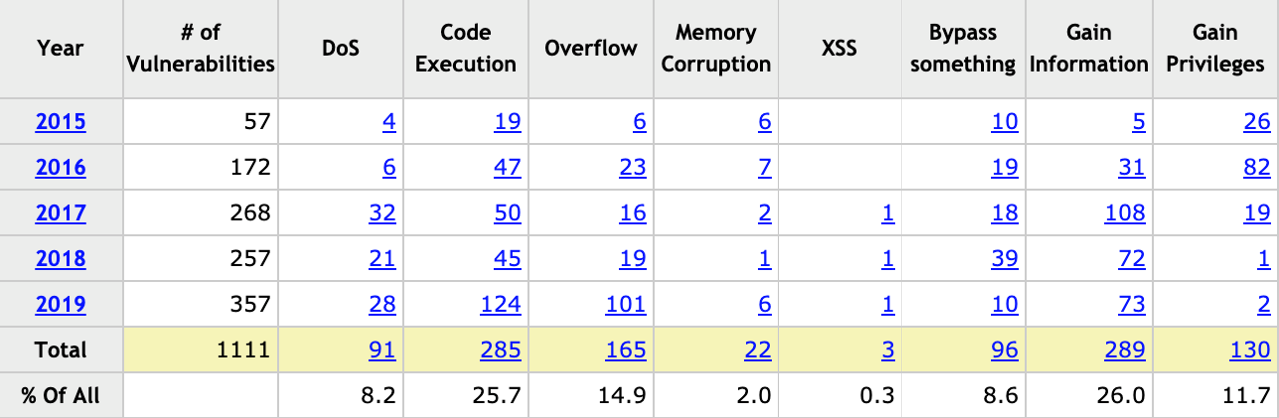
\includegraphics[width=8cm, height=2.5cm]{fig/stats}
\caption{Amount of documented vulnerabilities in the Windows Operating System.\newline Note that the spike in "Gain Information" vulnerabilities in 2017 is inflated by a family of attacks widely known as Meltdown/Spectre}
\end{figure}

We can see that the three largest groups of vulnerabilities consist of "Gain Information", "Code Execution" and "Overflow".
Of course these three categories aren't entirely seperated from each other.
An attacker that is able to execute Code on a machine often does so in order to gain information and overflows are often the reason why an attacker can execute code in the first place.
\section{Overflows}\label{sec:Overflows}
An overflow happens when a program writes data to memory beyond the limits of the intended data structure.

%\begin{figure}[htbp]
%  \centering
%  \fbox{\parbox{.8\columnwidth}{
%      Here you can include a sample figure.  Use something like
%      \begin{center}
%        \code{$\backslash$includegraphics[scale=.8]\{template\}}
%      \end{center}
%      to include an encapsulated postscript figure.  The \emph{scale}
%      argument can be used for scaling the picture, although it
%      may scale the font incorrectly.
%    }}
%  \caption{Sample Figure}
%  \label{fig:sample}
%\end{figure}


%\lstset{language=C, basicstyle=\ttfamily,
%        string=[b]', showspaces=false, showtabs=false,
%        caption={A sample code snippet}, captionpos=b}
%\begin{lstlisting}
%/* code snippet  */
%while (!sleep)
%	sleep++;
%\end{lstlisting}

%\begin{figure}[hbt]
%\centering
%\includegraphics[scale=.7,clip]{fig/OIUKAvV}
%\caption{Sample figure automatically from Windows prn.\label{plot:fig}}
%\end{figure}

\section{Related Work}\label{sec:relwork} 

\section{Approach}

\section{Conclusion}\label{sec:conclusion}

\bibliographystyle{abbrv}
\bibliography{Advanced Exploit Mitigation}
%\footnotesize
\end{document}
